% \subsection{Rotationsmatrizen}
%
% \begin{tabular}{ l | l }
% I & II \\ \hline
% IV & III \\
% \end{tabular}
%
% \flushleft
% \hfill
% \begin{tabular}{l | l l}
%   Clockwise & & \\ \hline
%   I & + & + \\
%   II & + & - \\
%   III & - & - \\
%   IV & - & +
% \end{tabular}
% \hfill
% \begin{tabular}{l | l l}
% Anticlockwise & & \\ \hline
% I & - & - \\
% II & - & + \\
% III & + & + \\
% IV & + & -
% \end{tabular}
% \hfill
%
% \subsection{Die Matrizen}
%
% \subsubsection{Rotation um die x-Achse}
%
% \begin{equation}
%   R_x (\alpha) =
%    \begin{pmatrix}
%       1 & 0 & 0 \\
%       0 & cos(\alpha) & -sin(\alpha) \\
%       0 & sin(\alpha) & cos(\alpha)
%     \end{pmatrix}
% \end{equation}
%
% \subsubsection{Rotation um die y-Achse}
%
% \begin{equation}
%   R_y (\alpha) =
%    \begin{pmatrix}
%       cos(\alpha) & 0 & sin(\alpha) \\
%       0 & 1 & 0 \\
%       -sin(\alpha) & 0 & cos(\alpha)
%     \end{pmatrix}
% \end{equation}
%
% \subsubsection{Rotation um die z-Achse}
%
% \begin{equation}
%   R_z (\alpha) =
%    \begin{pmatrix}
%       cos(\alpha) & -sin(\alpha) & 0 \\
%       sin(\alpha) & cos(\alpha) & 0 \\
%       0 & 0 & 1
%     \end{pmatrix}
% \end{equation}

\subsection{Spiralgalaxien}

\subsection{Using Object Oriented Programming (OOP) techniques}

In my case, the objects are galaxies.

\subsubsection{Initialisation}

The galaxy is initialised with the following objects:

\begin{itemize}
  \item A list storing the coordinates of each star
  \begin{itemize}
    \item X Coordinate
    \item Y Coordinate
    \item Z Coordinate
  \end{itemize}

  \item A list storing the individual forces acting on the stars
  \begin{itemize}
    \item X Force
    \item Y Force
    \item Z Force
  \end{itemize}

  \item A variable storing the number of stars generated in the galaxy

  \item Newtons gravitational constant
\end{itemize}

\subsection{Generation of new stars}

The function is given an integer defining the amount of stars that should be
newly generated.

The newly generated stars are then appended to the list storing the coordinates.

The counter counting the amount of stars in the galaxy is incremented.

\subsection{Printing all the coordinates}

The function cycles through the list storing the star coordinates and prints
them to the command line.

\subsection{Calculating the Forces acting between the Stars}

The function recieves two star objects and an axis on which the forces should
be calculated and returns the force acting on the given axis. In case of a
failture (The two given stars have got the same coordiantes), the function
just goes on to the next Star.

The Forces can be calculated using the equation (\ref{eq:gravitation_law}).

\subsection{Calculating the forces acting between each star in the galaxy and
each other star}

To calculate the forces inbetween every star in the galaxy, the function cycles
through every star, looks if the force that should be calculated hat not been
calculated yet and calculates it. This includes testing if the force that should
be calculated is not the force inbetween a star and itself.

The results of the calculations are stored in a list storinf the forces.

\subsection{Printing all the individual forces}

The function is able to print all the forces acting inbetween the stars if no
argument is given. If an argument n is given, the function print out the nth
star in the list.

\subsection{Spherical cells}


\subsubsection{Testing if a point is inside or outside a sphere}

In order to test is a point is inside a sphere, one just has to test if the
following conditions are all true:

\begin{equation}
  \begin{split}
    S_x - S_r \leq P_x \leq S_x + S_r \\
    S_y - S_r \leq P_y \leq S_y + S_r \\
    S_z - S_r \leq P_z \leq S_z + S_r
  \end{split}
\end{equation}

\( P_x \) , \( P_y \) and \( P_z \) are the coordinates of the point to be tested,
\( S_x \) , \( S_y \) and \( S_z \) are the coordinates of the midpoint of the sphere and
\( S_r \) is the radius of the sphere.

\subsubsection{Testing if a star is inside or outside of a sphere for a whole galaxy}

While testting if a star is inside a sphere or not, because of the alignment
of the spheres, a point can be in more than one sphere at the same time.
To get rid of this problem, the software cycles over every star and searches
for matches within the spheres. If a match is found, the next star is tested.
This is pretty much as efficient as it can get.

\begin{equation}
  O(n) = n_{stars} \cdot n_{spheres}
\end{equation}

\subsubsection{Generate the position of the spheres}

Generating the position of the spheres is accomplished in the following way:
A 3D-grid is generated and the midpoints of the spheres are positioned on the
gridpoints.

[Include Graphic]

The distance the spheres have to each other ist defined using the following
function:

\begin{equation} \label{sphere_distance}
  \texttt{sphere\_distance} = \frac{\texttt{galaxy\_range}}{\texttt{sampling\_rate}}
\end{equation}

The higher the \texttt{sampling\_rate} is, the more spheres get generated.

The next goal is to find out the ``sweet spot'' generating the spheres.
When using a very low \texttt{sampling\_rate}, the reault gets inacurate, but
when using a high \texttt{sampling\_rate}, the calculations are not affected
in term of speed and efficiency. The Goal is therefor to find a sampling rate
that enables the generation of accurate but fast results.

By being able to controll the accuracy anf therefor the time, it is possible to
teach the system to generate a galaxy in like one hour and it will automatically
set the sampling rate so low that the simulation will finish perfectly in time.

\subsubsection{The radius of the spheres}

The Radius of the spheres is dynamicly allocated to ensure that the whole galaxy
is covered.

\begin{equation} \label{sphere_radius}
  r = \sqrt{\texttt{sphere\_distance}^2 + \texttt{sphere\_distance}^2 + \texttt{sphere\_distance}^2}
\end{equation}

\begin{equation*}
  1.7320508075688772 = \sqrt{1^2 + 1^2 + 1^2}
\end{equation*}

The equation (\ref{sphere_radius}) highly depends on the equation
(\ref{sphere_distance}) and it's parameters.

\begin{figure}
  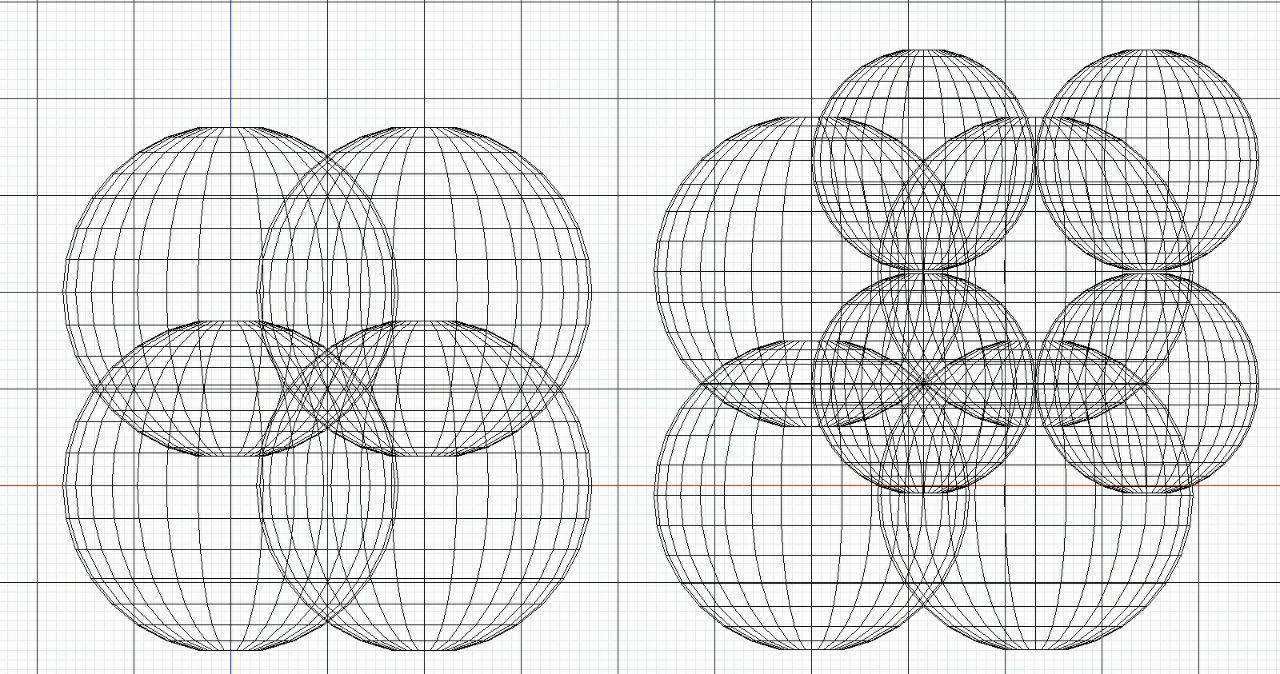
\includegraphics[width=1\textwidth]{figs/sphere_alignment_cc}
  \caption{The Alignment of the spheres\\
  Left: The perfect alignment covering the complete space\\
  Right: A previously generated alignment using small spheres to cover the missing space
  }
  \label{sphere_alignment}
\end{figure}

\subsubsection{Calculate the forces acting on the spheres}

In order to reduce the time that is needed to calculate the forces inbetween
the stars, the stars are subdivided in different cells, in this case spheres.
After all the forces acing inside one sphere are calculated, the forces are
combined and applied to the midpoint of the sphere genrating a new coordinate:
the mean force. The mean force inbetween all the cells can be calculated.

[Include description binary tree]

[Include graphic binary tree]

\subsubsection{Calculate the forces acting on all the spheres together}

This should be 0.

\subsubsection{Benchmarks}

\begin{tabular}{l | l | l | l}
  Nr of Stars & Sample rate & Galaxy Range & Time (s) \\\hline


  100         & 1           & 100          & 0.0814 \\
  75          & 1           & 100          & 0.0499 \\
  50          & 1           & 100          & 0.0295 \\
  25          & 1           & 100          & 0.0116 \\ \hline

  100         & 1           & 100          & 0.0828 \\
  100         & 2           & 100          & 0.0909 \\
  100         & 4           & 100          & 0.1832 \\
  100         & 8           & 100          & 1.1114 \\
  100         & 16          & 100          & 7.6944 \\
  100         & 32          & 100          & 56.5731 \\
  100         & 64          & 100          & 217.7768 \\ \hline

  100         & 1           & 1            & 0.0809 \\
  100         & 1           & 2            & 0.0844 \\
  100         & 1           & 4            & 0.0782 \\
  100         & 1           & 8            & 0.0758 \\
  100         & 1           & 16           & 0.0847 \\
  100         & 1           & 32           & 0.0815 \\
  100         & 1           & 64           & 0.0770 \\

\end{tabular}

The sample rate is the factor that influences the time the most. Knowing this,
it (the sample rate) can be used to controll the time in which a galaxy can
be created.
This is usefull in particular when using some very powerfull mashine with
limited time.

\subsection{Calculate the Position of a Star after a timestep}

Not to be considered:
\begin{itemize}
  \item drag
  \item any kind of resistance
  \item acceleration
\end{itemize}
